\section{Observations \& Calculation}

	All the graphs \hyperref[graph:1]{Figure 3}, \hyperref[graph:2]{Figure 4} and \hyperref[graph:3]{Figure 5} have been fitted in a straight line following the equation $y = mx+c$ where $m$ and $c$ are the parameters.
	\subsection{Germanium Sample}

		The Thickness of the provided Germanium sample was $0.5mm$. We plotted the potential difference measured with the current flowing through the sample as shown in \hyperref[tab:1]{Table 1} in \hyperref[graph:1]{Figure 3}. From the graph we can see that the slope of the curve is $slope = \sfrac{V}{I} = R = 87.94\pm0.05\ohm$.

		\begin{table}[h]
	\centering
	\begin{tabular}{|c|c|c|c|}
	\hline
	\textbf{\begin{tabular}[c]{@{}c@{}}Angle\\ $(\theta)$\end{tabular}} & \textbf{Time (s)} & \textbf{Counts} & \textbf{\begin{tabular}[c]{@{}c@{}}Counts per\\ second $N(\theta)$\end{tabular}} \\ \hline
	\multirow{5}{*}{25} & \multirow{5}{*}{600} & 133 & \multirow{5}{*}{0.225} \\ \cline{3-3}
	 &  & 140 &  \\ \cline{3-3}
	 &  & 127 &  \\ \cline{3-3}
	 &  & 137 &  \\ \cline{3-3}
	 &  & 138 &  \\ \hline
	\multirow{5}{*}{20} & \multirow{5}{*}{200} & 164 & \multirow{5}{*}{0.940} \\ \cline{3-3}
	 &  & 198 &  \\ \cline{3-3}
	 &  & 186 &  \\ \cline{3-3}
	 &  & 195 &  \\ \cline{3-3}
	 &  & 197 &  \\ \hline
	\multirow{5}{*}{15} & \multirow{5}{*}{100} & 311 & \multirow{5}{*}{2.929} \\ \cline{3-3}
	 &  & 276 &  \\ \cline{3-3}
	 &  & 277 &  \\ \cline{3-3}
	 &  & 311 &  \\ \cline{3-3}
	 &  & 290 &  \\ \hline
	\multirow{5}{*}{10} & \multirow{5}{*}{100} & 1726 & \multirow{5}{*}{17.626} \\ \cline{3-3}
	 &  & 1811 &  \\ \cline{3-3}
	 &  & 1713 &  \\ \cline{3-3}
	 &  & 1754 &  \\ \cline{3-3}
	 &  & 1809 &  \\ \hline
	\multirow{5}{*}{5} & \multirow{5}{*}{100} & 2931 & \multirow{5}{*}{29.286} \\ \cline{3-3}
	 &  & 2938 &  \\ \cline{3-3}
	 &  & 2912 &  \\ \cline{3-3}
	 &  & 2931 &  \\ \cline{3-3}
	 &  & 2931 &  \\ \hline
	\multirow{5}{*}{-5} & \multirow{5}{*}{100} & 2934 & \multirow{5}{*}{29.343} \\ \cline{3-3}
	 &  & 2933 &  \\ \cline{3-3}
	 &  & 2935 &  \\ \cline{3-3}
	 &  & 2935 &  \\ \cline{3-3}
	 &  & 2935 &  \\ \hline
	\multirow{5}{*}{-10} & \multirow{5}{*}{100} & 1751 & \multirow{5}{*}{17.824} \\ \cline{3-3}
	 &  & 1778 &  \\ \cline{3-3}
	 &  & 1831 &  \\ \cline{3-3}
	 &  & 1787 &  \\ \cline{3-3}
	 &  & 1766 &  \\ \hline
	\multirow{5}{*}{-15} & \multirow{5}{*}{100} & 291 & \multirow{5}{*}{2.940} \\ \cline{3-3}
	 &  & 294 &  \\ \cline{3-3}
	 &  & 289 &  \\ \cline{3-3}
	 &  & 290 &  \\ \cline{3-3}
	 &  & 306 &  \\ \hline
	\multirow{5}{*}{-20} & \multirow{5}{*}{200} & 210 & \multirow{5}{*}{1.009} \\ \cline{3-3}
	 &  & 194 &  \\ \cline{3-3}
	 &  & 211 &  \\ \cline{3-3}
	 &  & 201 &  \\ \cline{3-3}
	 &  & 194 &  \\ \hline
	\multirow{5}{*}{-25} & \multirow{5}{*}{600} & 133 & \multirow{5}{*}{0.225} \\ \cline{3-3}
	 &  & 140 &  \\ \cline{3-3}
	 &  & 127 &  \\ \cline{3-3}
	 &  & 135 &  \\ \cline{3-3}
	 &  & 141 &  \\ \hline
	\end{tabular}
	\caption{Table for $N(\theta)$ for 5mm thick Gold foil}
	\label{tab:1}
\end{table}
		
		\begin{figure}[h]
			\centering
			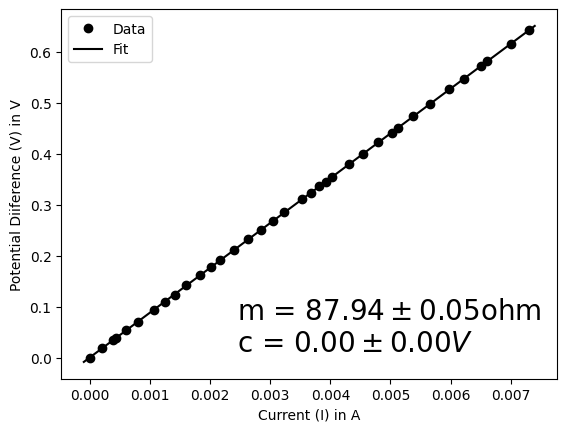
\includegraphics[width=0.8\columnwidth]{images/g1.png}
			\caption{V vs I graph for Germanium sample}
			\label{graph:1}
		\end{figure}

		So using \hyperref[eq:2]{Equation 2} we get the resistivity of the sample as:

		$$\rho_{Ge} = \frac{\pi}{\ln(2)}\times0.05\times87.94 = 19.93\;\ohm cm$$

	\subsection{Aluminium Sample}

		The Thickness of the provided Aluminium sample was $0.018mm$. We plotted the potential difference measured with the current flowing through the sample as shown in \hyperref[tab:2]{Table 2} in \hyperref[graph:2]{Figure 4}. From the graph we can see that the slope of the curve is $slope = \sfrac{V}{I} = R = 356.61\pm1.99\mu\ohm$.

		\begin{table}[H]
    \centering
    \begin{tabular}{|c|c|c|c|}
        \hline
        $V_{DC}$ & $V_{DUT}$ & $V_{OUT}$ & $C_{DUT}$   \\ \hline
        0        & 0.074     & 0.459     & 127.837 \\
        0.1      & 0.109     & 0.451     &  85.276 \\
        0.2      & 0.232     & 0.447     &  39.709 \\
        0.3      & 0.299     & 0.438     &  30.191 \\
        0.4      & 0.389     & 0.432     &  22.888 \\
        0.5      & 0.463     & 0.432     &  19.230 \\
        0.6      & 0.564     & 0.426     &  15.567 \\
        0.7      & 0.662     & 0.420     &  13.075 \\
        0.8      & 0.760     & 0.435     &  11.796 \\
        0.9      & 0.846     & 0.430     &  10.475 \\
        1        & 0.941     & 0.426     &   9.330 \\
        1.1      & 1.058     & 0.427     &   8.318 \\
        1.2      & 1.174     & 0.422     &   7.408 \\
        1.3      & 1.267     & 0.418     &   6.799 \\
        1.4      & 1.357     & 0.416     &   6.318 \\
        1.5      & 1.464     & 0.412     &   5.800 \\
        1.6      & 1.559     & 0.409     &   5.406 \\ \hline
    \end{tabular}
    \caption{Data for light condition}
    \label{tab:2}
\end{table}
		
		\begin{figure}[h]
			\centering
			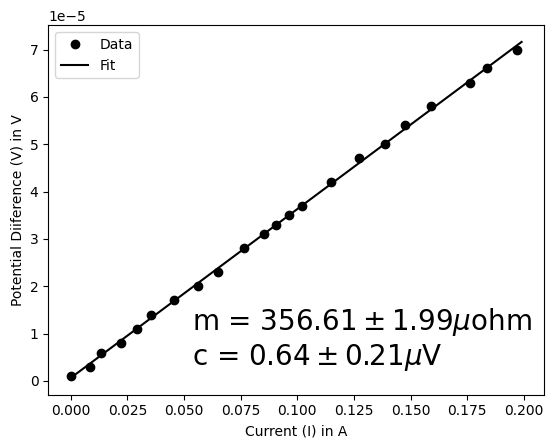
\includegraphics[width=0.8\columnwidth]{images/g2.png}
			\caption{V vs I graph for Aluminium sample}
			\label{graph:2}
		\end{figure}

		So using \hyperref[eq:2]{Equation 2} we get the resistivity of the sample as:

		$$\rho_{Al} = \frac{\pi}{\ln(2)}\times0.0018\times356.61\times10^{-6} = 2.91\times10^{-6}\;\ohm cm$$

	\subsection{Silicon Sample}

		The Thickness of the provided Silicon sample was $0.5mm$. We plotted the potential difference measured with the current flowing through the sample as shown in \hyperref[tab:3]{Table 3} in \hyperref[graph:3]{Figure 5}. From the graph we can see that the slope of the curve is $slope = \sfrac{V}{I} = R = 105.06\pm0.71\ohm$.

		\begin{table}[]
	\centering
	\begin{tabular}{|l|l|}
	\hline
		H(gauss) & V(mV) \\ \hline
		2390 & -0.061 \\ \hline
		2540 & -0.062 \\ \hline
		3160 & -0.063 \\ \hline
		3480 & -0.064 \\ \hline
		4200 & -0.065 \\ \hline
		4500 & -0.066 \\ \hline
		4780 & -0.067 \\ \hline
		5200 & -0.068 \\ \hline
		5180 & -0.069 \\ \hline
	\end{tabular}
	\caption{Magnetoresistance Data for $I=101.0mA$}
	\label{tab:mag2}
\end{table}
		
		\begin{figure}[h]
			\centering
			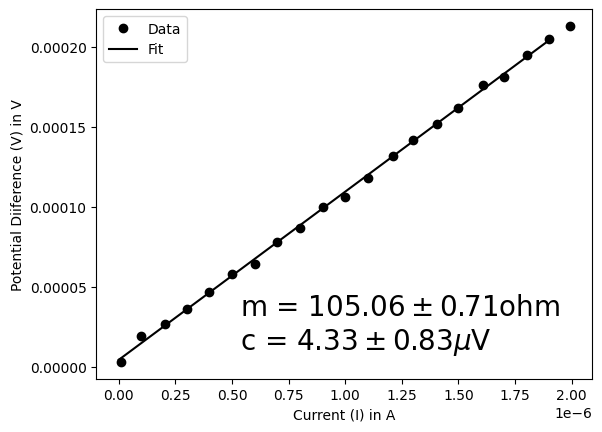
\includegraphics[width=0.8\columnwidth]{images/g3.png}
			\caption{V vs I graph for Aluminium sample}
			\label{graph:3}
		\end{figure}

		So using \hyperref[eq:2]{Equation 2} we get the resistivity of the sample as:

		$$\rho_{Al} = \frac{\pi}{\ln(2)}\times0.05\times105.06 = 23.8\;\ohm cm$$

	\subsection{Germanium with Varying Temperature}

		We measured the potential difference between the two probes of the germanium sample at different temperatures. The current was kept constant at $0.5mA$. The data is shown in \hyperref[tab:4]{Table 4}. From the data, we plotted the graph between $\log\rho$ and $1/T$ as shown in \hyperref[graph:4]{Figure 6}.

		\begin{table}[h]
	\centering
	\resizebox{\columnwidth}{!}{%
		\begin{tabular}{|c|c|c|c|c|c|}
			\hline
			\textbf{Source}                      & \textbf{Distance (cm)} & \textbf{Counts} & \textbf{Corrected Counts} & \textbf{Average}         & \multicolumn{1}{l|}{\textbf{CPS}} \\ \hline
			\multirow{3}{*}{\textbf{$Cs^{137}$}} & \multirow{3}{*}{10}    & 738             & 655                       & \multirow{3}{*}{670.667} & \multirow{3}{*}{11.178}           \\ \cline{3-4}
			                                     &                        & 766             & 683                       &                          &                                   \\ \cline{3-4}
			                                     &                        & 757             & 674                       &                          &                                   \\ \hline
			\multirow{3}{*}{\textbf{$Tl^{204}$}} & \multirow{3}{*}{2}     & 2306            & 2223                      & \multirow{3}{*}{2224}    & \multirow{3}{*}{37.067}           \\ \cline{3-4}
			                                     &                        & 2309            & 2226                      &                          &                                   \\ \cline{3-4}
			                                     &                        & 2306            & 2223                      &                          &                                   \\ \hline
		\end{tabular}%
	}
	\caption{Efficiency Data}
	\label{tab:4}
\end{table}
		
		\begin{figure}[h]
			\centering
			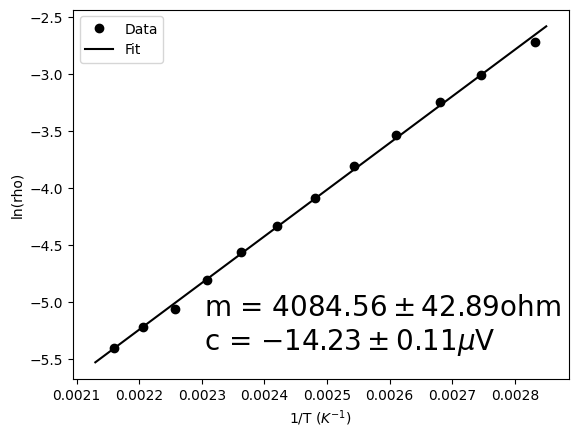
\includegraphics[width=0.8\columnwidth]{images/g4.png}
			\caption{V vs I graph for Germanium sample}
			\label{graph:4}
		\end{figure}

		From \hyperref[graph:4]{Figure 6} we can see that the slope of the straight line is $4084.56\pm42.89\ohm$. Using \hyperref[eq:3]{Equation 3} we get the band gap of the germanium sample as:

		\begin{equation}
			\begin{split}
				E_g &= 2\times k_B\times slope\\
				&= 2\times8.6\times10^{-5}\times 4084.56 eV\\
				&= 0.703 eV
			\end{split}
		\end{equation}
		
